\newpage
\section{Потоки сообщений EAP-PSK}

EAP-PSK включает в себя два различных типа потоков сообщений:

\begin{itemize}
\item Стандартная аутентификация:
\begin{itemize}
\item обязательна к реализации;
\item полностью описана в данном документе;
\item простейший тип потока сообщений, который, как ожидается, будет использоваться наиболее часто.
\end{itemize}
\item Расширенная аутентификация:
\begin{itemize}
\item Не обязательна к реализации;
\item Частично описана в данном документе, поскольку сильно зависит от расширений, не указанных в данном документе;
\item Тип потока сообщений, использующийся при расширении протокола EAP-PSK если от него требуются дополнительные функции.
\end{itemize}
\end{itemize}

EAP-PSK использует концепцию сессий для более легкого анализа протокла и обеспечения прозарчного интерфейса для других уровней. Сессией называется EAP-PSK взаимодействие между двумя сторонами. Каждая сессия определяется её идентификатором.

EAP сервер устанавлиает идентификатор сессии в первом EAP-PSK сообщении. Учитывая тот факт, что EAP-Request/Identity и EAP-Responce/Identity не могут предпологать, что происходило до их отправки и что данные, пересылаемые в EAP-Responce/Identity (Если такой запрос производился) может не содержать актуального NAI который Пир должен использовать с EAP-PSK мы приходим к тому, что EAP сервер, использующий метод EAP-PSK должен использовать один и тот же NAI сервера EAP для всех EAP-PSK сессий с любыми Пирами, поддерживающими EAP-PSK.

\subsection{Стандартная аутентификация EAP-PSK}

Стандартная аутентификация EAP-PSK состоит из четырех сообщений, то есть двух раундов, представленных на рисунке \ref{img:standart_aut}.

\begin{figure}[h!]
\center{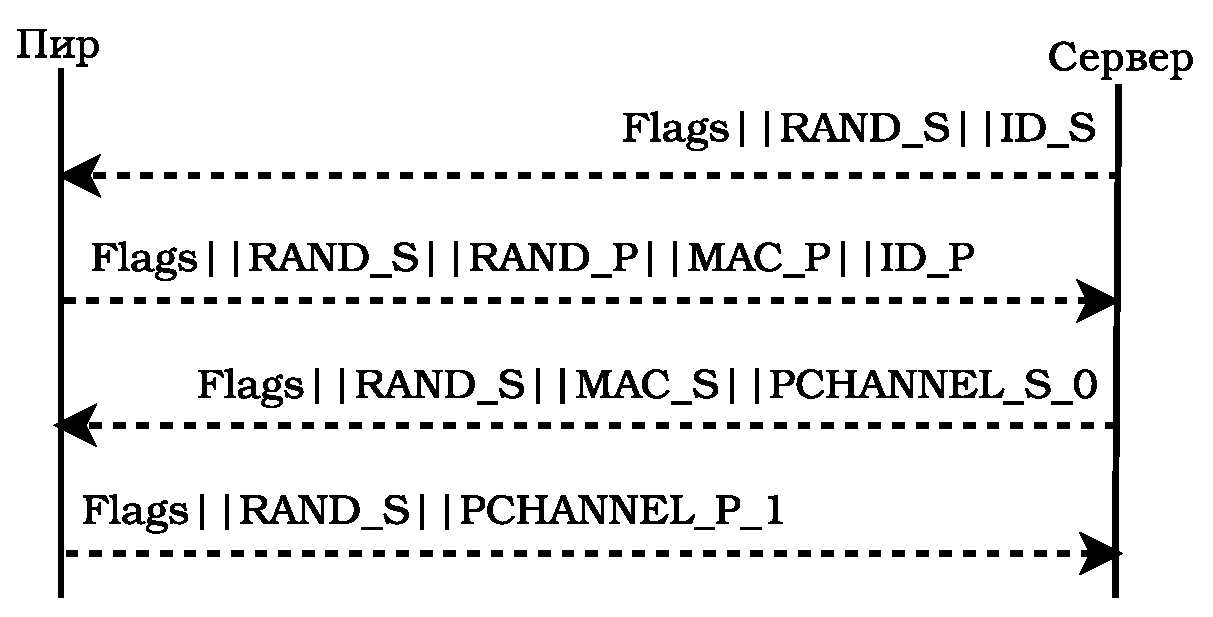
\includegraphics[width=0.9\linewidth]{./pictures/standart_aut}}
\caption{Стандартная аутентификация EAP-PSK}
\label{img:standart_aut}
\end{figure}
